Khối điều khiển (Controller) tiếp nhận, xử lý và điều phối các tín hiệu kích hoạt cho quá trình nạp lệnh và thực thi lệnh. 
Controller được thiết kế đồng bộ theo xung lên của (\texttt{clk}) và sử dụng máy trạng thái hữu hạn (Finite State Machine - FSM) 
gồm 8 pha hoạt động liên tục.

\begin{figure}[H]
    \centering
    % Đảm bảo file ảnh nằm cùng thư mục với file .tex. Thay đổi tên file nếu cần.
    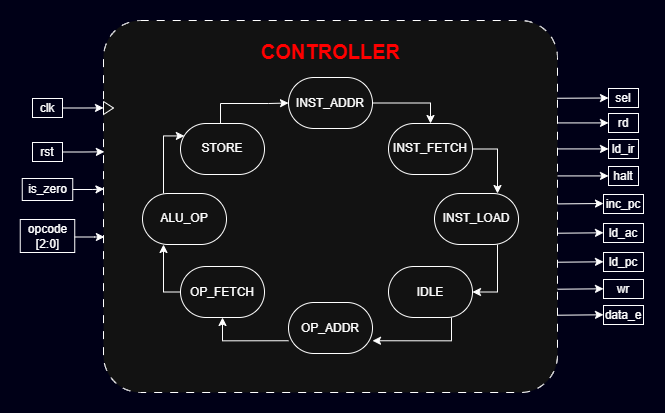
\includegraphics[width=0.75\textwidth]{Controller.png} 
    \caption{Sơ đồ khối và máy trạng thái 8 pha của Controller}
    \label{fig:controller_diagram}
\end{figure}

\textbf{Các tín hiệu bao gồm:}

\begin{itemize}
    \item \textbf{Tín hiệu vào (Inputs): }
    \begin{itemize}
        \item \textbf{\texttt{opcode [2:0]}: } Mã lệnh 3-bit nhận từ khối \texttt{IR}. 
        Dữ liệu được Controller giải mã và quyết định thao tác thực thi trong các pha tiếp theo.
        \item \textbf{\texttt{is\_zero}: } Cờ trạng thái từ khối ALU, tích cực khi kết quả tính toán bằng 0. 
        Tín hiệu này kết hợp với mã lệnh \texttt{SKZ} để quyết định việc rẽ nhánh.
        \item \textbf{\texttt{clk}: } Xung nhịp đồng bộ.
        \item \textbf{\texttt{rst}: } Đưa Controller về trạng thái ban đầu.
    \end{itemize}
    
    \item \textbf{Tín hiệu ra (Outputs):}
    \begin{itemize}
        \item \textbf{Nhóm Định tuyến và Bộ nhớ:} \texttt{sel} (Chọn địa chỉ từ \texttt{PC} hoặc \texttt{IR}), \texttt{rd} (Cho phép đọc từ Memory), 
        \texttt{wr} (Cho phép ghi vào Memory), \texttt{data\_e} (Cho phép dữ liệu từ Accumulator đi vào bus).
        \item \textbf{Nhóm Thanh ghi:} \texttt{ld\_ir} (Cho phép lệnh đi vào IR), \texttt{ld\_ac} (Cho dữ liệu đi vào Accumulator), 
        \texttt{ld\_pc} (Cho phép nạp địa chỉ vào PC), \texttt{inc\_pc} (Tăng giá trị PC).
        \item \textbf{Tín hiệu dừng:} \texttt{halt} (Dừng toàn bộ hoạt động của CPU).
    \end{itemize}
\end{itemize}

\textbf{Nguyên lý hoạt động của Máy trạng thái (FSM):}

Hệ thống hoạt động theo một vòng lặp khép kín gồm 8 pha, 
bắt đầu từ trạng thái reset là \texttt{INST\_ADDR}. Quá trình được chia làm hai giai đoạn chính:

\begin{enumerate}
    \item \textbf{Giai đoạn Nạp lệnh (Fetch Phase):} Bao gồm 4 trạng thái đầu tiên: \texttt{INST\_ADDR}, \texttt{INST\_FETCH}, \texttt{INST\_LOAD}, và \texttt{IDLE}. 
    \begin{itemize}
        \item Trong suốt giai đoạn này, tín hiệu \texttt{sel = 1} được giữ cố định để địa chỉ đi từ PC tới bộ nhớ.
        \item Bộ nhớ được phép đọc (\texttt{rd = 1}) và lệnh được đưa vào IR (\texttt{ld\_ir = 1}) ở các pha tương ứng.
    \end{itemize}
    
    \item \textbf{Giai đoạn Thực thi (Execute Phase):} Bao gồm 4 trạng thái cuối: \texttt{OP\_ADDR}, \texttt{OP\_FETCH}, \texttt{ALU\_OP}, và \texttt{STORE}.
    \begin{itemize}
        \item Tín hiệu \texttt{sel} chuyển về \texttt{0} để sử dụng phần địa chỉ chứa trong câu lệnh hiện tại.
        \item Tại \texttt{OP\_ADDR}, tín hiệu \texttt{inc\_pc} được kích hoạt bằng \texttt{1} để trỏ sẵn PC tới lệnh kế tiếp.
        \item Các ngõ ra trong các pha tiếp theo phụ thuộc vào bộ giải mã lệnh (\texttt{opcode}):
        \begin{itemize}
            \item Các lệnh tính toán (\texttt{ADD, AND, XOR, LDA}) sẽ kích hoạt \texttt{rd = 1} để lấy toán hạng và \texttt{ld\_ac = 1} tại pha \texttt{STORE} để lưu kết quả.
            \item Lệnh nhảy (\texttt{SKZ}) sẽ kiểm tra cờ \texttt{zero}. Nếu \texttt{zero = 1}, 
            tín hiệu \texttt{inc\_pc} sẽ được kích hoạt thêm một lần nữa tại pha \texttt{ALU\_OP}.
            \item Lệnh lưu dữ liệu (\texttt{STO}) sẽ kích hoạt \texttt{wr = 1} và \texttt{data\_e = 1} tại pha \texttt{STORE} để đẩy dữ liệu từ Accumulator vào bộ nhớ.
            \item Lệnh dừng (\texttt{HLT}) kích hoạt tín hiệu \texttt{halt = 1} ngay tại pha \texttt{OP\_ADDR}.
        \end{itemize}
    \end{itemize}
\end{enumerate}